\section{Principal Component Analysis}

For doing the principal component analysis, the data have been standardized.

\subsection{Variance explained by Principal Components}

In Figure \ref{VariancePCA}, we can see how the variance is explained by the principal component. We can see that the first principal component explains 32\% of the variance, while the second component explains 13\% of the variance. This means that we can explain 45\% of the total variance by using the two first principal components. Furthermore one can see from the graph that we need 5 principal components in order to explain 75\% of the variance, and at least 7 components to explain 90\% of the variance.

\begin{figure}[H]
\centering
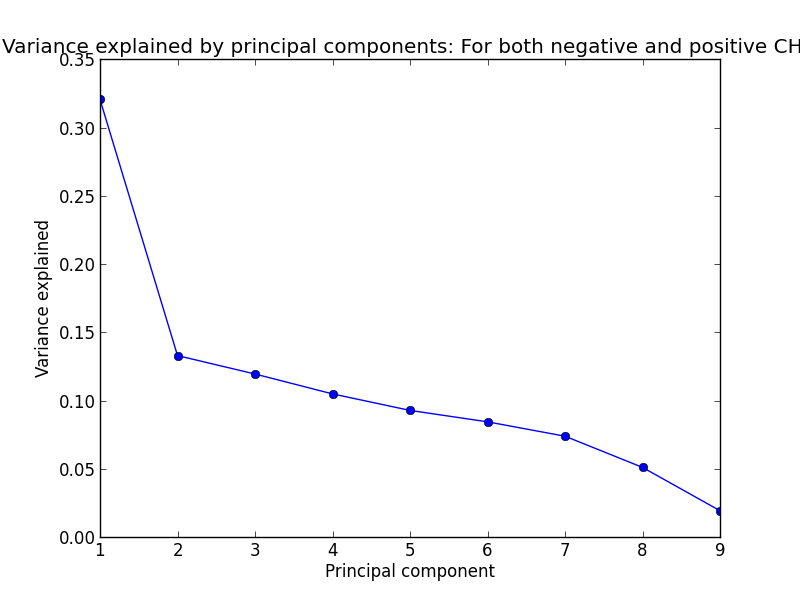
\includegraphics[width=7cm, keepaspectratio=true]{pictures/PCAPosAndNeg.png}
\caption{Showing how the variance is explained by the principal components.}
\label{VariancePCA}
\end{figure}

\subsection{Direction of the principal components}

Below in Figure \ref{PCADirections}, we can see the directions of the principal components. The most interesting components are the first ones, as these describe the biggest part of the variance. Looking at the first principal component, we see that obesity, adiposity and age are very relevant, while the most dominant attributes in the second principal component are alcohol and tobacco. We see that all the attributes effect the principal components, meaning they all have impact, however some attributes have larger impact than others. Eg. typea and family history are not heavily described by the first two principal components.

\begin{figure}[H]
\begin{longtable}{ l c c c c c c c c c}
 \hline
 \emph{Attributes} &  \emph{sbp} &  \emph{tobacco} &  \emph{ldl} & \emph{adiposity} &  \emph{famhist} &  \emph{typea} &  \emph{obesity} &  \emph{alcohol} &  \emph{age} \\ \hline
PC1 & -0.3238 & -0.3018 &  -0.3339 &  -0.5163 & -0.1951 & 0.0183 & -0.4015 & -0.1214 & -0.4601 \\ 
PC2 & 0.2383 &  0.4585 & -0.3639 &  -0.1876 &  0.0013 &   -0.2822 & -0.3919 & 0.5430 & 0.1930 \\ 
PC3 & -0.1251 & 0.0682 &  0.0031 & -0.0819 &  0.3384 & 0.7923 & 0.0402 &  0.4591 & -0.1353 \\ 
PC4 & -0.1964 & 0.0054 & 0.1403 & -0.1350 &  0.8334 & -0.2098 & -0.3055 & -0.2585 &  0.1573 \\ 
PC5 & 0.2149 & -0.6236 & -0.2422 &  0.1189 &  0.3054 & -0.3210 & 0.2834 &  0.4190 &  -0.1999 \\ 
PC6 & -0.7814 &  0.1631 &   0.2153 &  0.1309 & -0.0857 & -0.3319 & 0.1736 & 0.3793 & -0.0887 \\ 
PC7 & -0.2681 &  0.1929 & -0.7882 &  0.1957 &  0.1285 &  0.0778 & 0.3333 & -0.2768 &  0.1453 \\ 
PC8 & 0.2354 &  0.4889 &  0.0703 & -0.1731 & 0.1866 & -0.1655 &   0.3387 & -0.1251 & -0.6914 \\ 
PC9 & -0.0141 & -0.0478 & 0.0719 & -0.7575 & -0.0288 & -0.0406 & 0.5040 & 0.0331 & 0.4012 \\ \hline  
\end{longtable}
\caption{Describing the directions of the principal components.}
\label{PCADirections}
\end{figure}

\subsection{Projection of data onto Principal Components}

We can see the data projected onto the first two principal components in Figure \ref{PCAProjected}. At first glance it is hard to see a pattern. However one can see that most of the sick people are located in a direction, where the first principal component is negative. By comparing to how the attributes are described in this component, as shown in Figure \ref{PCADirections}, we see that this principal component are pointing in the negative direction for all the attributes, except typea which is hardly described in this component. And since we have a lot of ill subjects in this negative direction of principal component 1, it indicates that these people have high values in these attributes. Meaning these subjects have a tendency to have high adiposity for instance. The data has been standardized for doing this principal component analysis, meaning that Figure \ref{PCAProjected} indicates that many of the ill subjects has values above the mean in most attributes.

\begin{figure}[H]
\centering
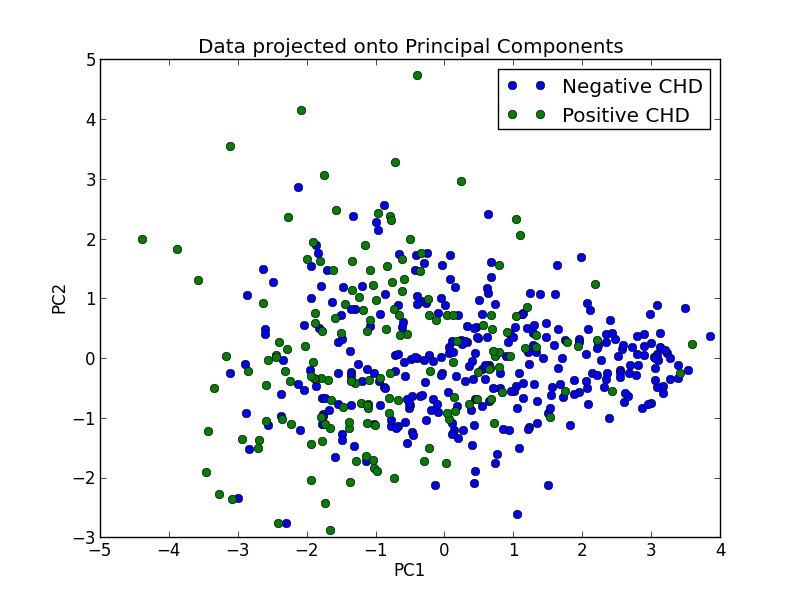
\includegraphics[width=7cm, keepaspectratio=true]{pictures/projectedToPCA.png}
\caption{Projection of data onto first two principal components.}
\label{PCAProjected}
\end{figure}